\part{集群方案篇}

本章介绍几种高可用的解决方案。

\chapter{集群基础知识}

\section{集群概述}

集群是一组协同工作的服务实体,用以提供比单一服务实体更具扩展性和可用性
的服务平台。

在客户端看来,一个集群就是一个完整不可细分的实体,但事实上一个集群实体
是由完成不同任务的服务节点个体所组成的。

集群实体的可扩展性是指,在集群运行中新的服务节点可以动态的加入集群实体
从而提升集群实体的综合性能。

集群实体的高可用性是指,集群实体通过其内部的服务节点的冗余使客户端免于
OUT OF SERVICE错误。简单的说,在集群中同一服务可以由多个服务节点提供,
当部分服务节点失效后,其他服务节点可以接管服务。

集群实体地址是指客户端访问集群实体获得服务资源的唯一入口地址。

负载均衡是指集群中的分发设备(服务)将用户的请求任务比较均衡(不是平均)
分发到集群实体中的服务节点计算、存储和网络资源中。一般我们将提供负载均
衡分发的设备叫做负载均衡器。负载均衡器一般具备如下三个功能:

\begin{enumerate}[itemsep=0pt,parsep=0pt]
\item 维护集群地址
\item 负责管理各个服务节点的加入和退出
\item 集群地址向内部服务节点地址的转换
\end{enumerate}

错误恢复是指集群中某个节点或某些服务节点(设备)不能正常工作(或提供服
  务),其他类似服务节点(设备)可以资源透明和持续的完成原有任务。具备
错误恢复能力是集群实体高可用性的必要条件。

负载均衡和错误恢复都需要集群实体中各个服务节点中有执行同一任务的资源存
在,而且对于同一任务的各个资源来说,执行任务所学的信息视图必须一致。

\section{集群类型}

多台同构或异构的计算机用某种方式连接起来协同完成特定的任务就构成了集群
系统,目前Linux下的集群主要有三种类型:

\begin{enumerate}[itemsep=0pt,parsep=0pt]
\item HA(High Availability)
\item LB(Load Balancing)
\item HPC(High Performance Computing)
\end{enumerate}

\chapter{Keepalived}
\label{chap:keepalived}

\section{Keepalived简介}

KeepAlived起初是专为LVS设计的,专门用来监控LVS集群系统中各个服务节点的
状态,后来又加入了VRRP的功能,因此,除了配合LVS服务外,也可以作为其他服
务(如Nginx,HAProxy等)的高可用软件。VRRP是Virtual Router Redundancy
Protocol(虚拟路由冗余协议)的缩写,VRRP出现的目的就是为了解决静态路由
出现的单点故障问题,它能够保证网络的不间断、稳定地运行。所
以,KeepAlived一方面具有LVS cluster nodes healthcheck功能,另一方面也具
有LVS directors failover功能。

\section{Keepalived安装部署}

\subsection{环境准备}

演示环境为CentOS6.5 64位系统,机器列表如下:

\begin{table}[!htbp]
  \centering
  \caption{KeepAlived演示环境机器列表}
  \begin{tabular}{|l|l|r|}
    \hline
    主机名  & IP地址 & 角色 \\
    \hline
    lb01.lavenliu.com & 192.168.20.150 & KeepAlived(主) \\
    \hline
    lb02.lavenliu.com & 192.168.20.151 & KeepAlived(备) \\
    \hline
  \end{tabular}
\end{table}

\subsection{开始安装}

\begin{verbatim}
yum install -y keepalived
\end{verbatim}

\subsection{Keepalived配置介绍}

\section{运行服务与故障模拟}


\chapter{LVS+Keepalived负载均衡集群}

LVS(Linux Virtual Server) is a cluster of servers 

The Linux Virtual Server can be used to build scalable network
services based on a cluster of two or more nodes. The active node of
the cluster redirects service requests to a collection of server hosts
that will actually perform the services. Supported features include
two protocols (TCP and UDP), three packet-forwarding methods (NAT,
tunneling, and direct routing), and eight load balancing algorithms
(round robin, weighted round robin, least-connection, weighted
least-connection, locality-based least-connection, locality-based
least-connection with replication, destination-hashing, and
source-hashing).

LVS: ipvsadm/ipvs

When a new connection is requested from a client to a service provided
by the LVS (e.g. httpd), the director will choose a realserver from
the client.

From then, all packets from the client will go through the director to
that particular realserver.

The association between the client and the realserver will last for
only the life of the tcp connection (or udp exchange).

For the next tcp connection, the director will choose a new realserver
(which may or may not be the same as the first realserver).

Thus a web browser connecting to a LVS serving a webpage consisting of
several hits (images, html page), may get each hit from a separate
realserver.

LVS IP Address Name Conventions

Virtual IP (VIP) address: The IP address the Director uses to offer
services to client computers

Real IP (RIP) address: The IP address used on the cluster nodes

Director's IP (DIP) address: The IP address the Director uses to
connect to the D/RIP network

Client computer's IP (CIP) address: The IP address assigned to a
client computer that it uses as a source IP address for requests sent
to the cluster

\begin{quote}
  Basic Properties of LVS-NAT 

1. The cluster nodes need to be on the
same network (VLAN or subnet) as the Director.
集群节点必须与调度器在同一个网络中


2. The RIP addresses of the cluster nodes are normally private,
non-routable IP addresses used only for intracluster communication.
RIP通常是私有地址,仅用于各集群节点间的通信

3. director位于client与real server之间,并负责处理进出的所有通信

4. realserver必须将网关指向DIP

5. 支持端口映射

6. real server可以使用任何操作系统

7. 较大规模应用场景中,director易成为系统瓶颈
\end{quote}

\begin{quote}
  1. 集群节点跟director必须在同一物理网络中

  2. RIP可以使用公网地址,实现便捷的远程管理和监控

  3. director仅负责处理入站请求,响应报文则由real server直接发往客户端

  4. real server不能讲网关指向DIP

  5. 不支持端口映射

  real server必须能够隐藏VIP
\end{quote}

\begin{quote}
  TUN:
  1. 集群节点可以跨越Internet
  2. RIP必须是公网地址
  3. Director仅处理入站请求,响应报文则由real server直接发往客户端
  4. real server网关不能指向director
  5. 只有支持隧道功能的os才能用于real server
  6. 不支持端口映射
\end{quote}

\section{LVS调度算法}

Director在接收到来自于Client的请求时,会基于"schedule"从RealServer中选
择一个响应给Client。ipvs支持以下调度算法:

\begin{enumerate}[itemsep=0pt,parsep=0pt]
\item 轮询(round robin, rr),加权轮询(Weighted round robin, wrr)

  新的连接请求被轮流分配至各RealServer;算法的优点是其简洁性,它无需记
  录当前所有连接的状态,所以它是一种无状态调度。轮叫调度算法假设所有服
  务器处理性能均相同,不管服务器的当前连接数和响应速度。该算法相对简单,
  不适用于服务器组中处理性能不一的情况,而且当请求服务时间变化比较大时,
  轮叫调度算法容易导致服务器间的负载不平衡。

\item 最少连接(least connected, lc), 加权最少连接(weighted least
  connection, wlc)

  新的连接请求将被分配至当前连接数最少的RealServer;最小连接调度是一种
  动态调度算法,它通过服务器当前所活跃的连接数来估计服务器的负载情况。
  调度器需要记录各个服务器已建立连接的数目,当一个请求被调度到某台服务
  器,其连接数加1;当连接中止或超时,其连接数减一。

\item 基于局部性的最少链接调度(Locality-Based Least Connections
  Scheduling,lblc)

  针对请求报文的目标IP地址的负载均衡调度,目前主要用于Cache集群系统,因
  为在Cache集群中客户请求报文的目标IP地址是变化的。这里假设任何后端服务
  器都可以处理任一请求,算法的设计目标是在服务器的负载基本平衡情况下,
  将相同目标IP地址的请求调度到同一台服务器,来提高各台服务器的访问局部
  性和主存Cache命中率,从而整个集群系统的处理能力。LBLC调度算法先根据请
  求的目标IP地址找出该目标IP地址最近使用的服务器,若该服务器是可用的且
  没有超载,将请求发送到该服务器;若服务器不存在,或者该服务器超载且有
  服务器处于其一半的工作负载,则用“最少链接”的原则选出一个可用的服务
  器,将请求发送到该服务器。

\item 带复制的基于局部性最少链接调度(Locality-Based Least Connections
  with Replication Scheduling,lblcr)

  也是针对目标IP地址的负载均衡,目前主要用于Cache集群系统。它与LBLC算法
  的不同之处是它要维护从一个目标IP地址到一组服务器的映射,而 LBLC算法维
  护从一个目标IP地址到一台服务器的映射。对于一个“热门”站点的服务请求,
  一台Cache 服务器可能会忙不过来处理这些请求。这时,LBLC调度算法会从所
  有的Cache服务器中按“最小连接”原则选出一台Cache服务器,映射该“热
  门”站点到这台Cache服务器,很快这台Cache服务器也会超载,就会重复上述
  过程选出新的Cache服务器。这样,可能会导致该“热门”站点的映像会出现在
  所有的Cache服务器上,降低了Cache服务器的使用效率。LBLCR调度算法将“热
  门”站点映射到一组Cache服务器(服务器集合),当该“热门”站点的请求负
  载增加时,会增加集合里的Cache服务器,来处理不断增长的负载;当该“热
  门”站点的请求负载降低时,会减少集合里的Cache服务器数目。这样,该“热
  门”站点的映像不太可能出现在所有的Cache服务器上,从而提供Cache集群系
  统的使用效率。LBLCR算法先根据请求的目标IP地址找出该目标IP地址对应的服
  务器组;按“最小连接”原则从该服务器组中选出一台服务器,若服务器没有
  超载,将请求发送到该服务器;若服务器超载;则按“最小连接”原则从整个
  集群中选出一台服务器,将该服务器加入到服务器组中,将请求发送到该服务
  器。同时,当该服务器组有一段时间没有被修改,将最忙的服务器从服务器组
  中删除,以降低复制的程度。

\item 目标地址散列调度(Destination Hashing,dh)

  算法也是针对目标IP地址的负载均衡,但它是一种静态映射算法,通过一个散
  列(Hash)函数将一个目标IP地址映射到一台服务器。目标地址散列调度算法
  先根据请求的目标IP地址,作为散列键(Hash Key)从静态分配的散列表找出
  对应的服务器,若该服务器是可用的且未超载,将请求发送到该服务器,否则
  返回空。

\item 源地址散列调度(Source Hashing,sh)

  算法正好与目标地址散列调度算法相反,它根据请求的源IP地址,作为散列键
  (Hash Key)从静态分配的散列表找出对应的服务器,若该服务器是可用的且
  未超载,将请求发送到该服务器,否则返回空。它采用的散列函数与目标地址
  散列调度算法的相同。除了将请求的目标IP地址换成请求的源IP地址外,它的
  算法流程与目标地址散列调度算法的基本相似。在实际应用中,源地址散列调
  度和目标地址散列调度可以结合使用在防火墙集群中,它们可以保证整个系统
  的唯一出入口。
\end{enumerate}


基于DNS的负载均衡方案性能可能会出现问题。DNS的记录会缓存。

rsync基于文件的同步,效率低。

drbd磁盘镜像,让两个计算机的两块磁盘做镜像,基于块级别的同步,效率高。

\section{安装LVS}
\label{installLVS}

\subsection{环境准备}
\label{sec:lvsEnvPrepare}



\chapter{Heartbeat高可用集群}

Heartbeat提供了诸多集群基础架构服务,比如集群之间的消息传递、节点成员
身份、IP地址分配和迁移,以及服务的开启和停止。Heartbeat可以用来为
Apache、Samba和Squid等企业应用系统构建几乎任何一种高可用性的集群。此外,
它可以结合负载均衡软件使用,那样入站请求就可以由所有集群节点来分担。

本文中的示例集群将由2台运行Heartbeat的服务器组成。我们测试故障切换机
制的方法是,手动关闭服务器,检查它们服务的网站是不是仍然可用。下面是我
们的测试拓扑结构:

\begin{figure}[!htbp]
  \centering
  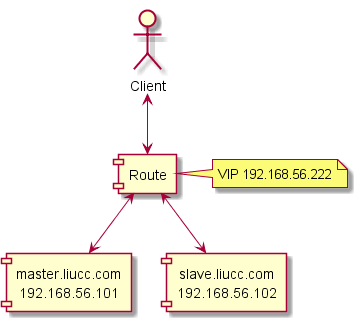
\includegraphics[width=0.5\textwidth]{img/heartbeat.png}
  \caption{heartbeat实验拓扑}
\end{figure}

映射服务所用的IP地址需要一直能够访问得到。通常,Heartbeat会为你将指定
的IP地址分配给主服务器上的虚拟网络接口卡。如果主服务器出现了故障,集群
会自动将IP地址切换到另一台可用服务器上的虚拟网卡。如果主服务器恢复正常
运行,它会再次将IP地址切换回到主服务器。由于具有迁移属性,这个IP地址被
称为“浮动”地址。

\section{安装Heartbeat}

在所有服务器上安装软件包

想组建集群,首先要使用yum,在每一个节点上安装必要的软件包:

\begin{verbatim}
yum install PyXML cluster-glue cluster-glue-libs resource-agents
\end{verbatim}

下一步,下载和安装官方CentOS软件库里面没有的两个Heartbeat RPM文件。

另外,你可以将EPEL软件库添加到源文件,并使用yum进行安装。

Heartbeat会管理Apache的httpd服务的开启和停止,所以停止Apache,并禁止它自动开启:

\begin{verbatim}
service httpd stop
chkconfig httpd off
\end{verbatim}

设置主机名称

现在设置服务器的主机名称,为此编辑每个系统上的/etc/sysconfig/network,并更改HOSTNAME这一行:

HOSTNAME=xxxxx.liucc.com 新的主机名称会在服务器下一次启动时激活。
你可以使用hostname命令立即激活它,不需要重启服务器:

hostname xxxxx.liucc.com 你可以在每一台服务器上运行uname -n,以此证实主机名称已正确设置好。

\section{配置Heartbeat}

想配置Heartbeat,首先要将其默认配置文件从/usr拷贝到/etc/ha.d/:

\begin{verbatim}
cp /usr/share/doc/heartbeat-3.0.4/authkeys /etc/ha.d/
cp /usr/share/doc/heartbeat-3.0.4/ha.cf /etc/ha.d/
cp /usr/share/doc/heartbeat-3.0.4/haresources /etc/ha.d/
\end{verbatim}

然后,你还得改动全部集群节点上的所有三个文件,以便与你的需求相匹配。

authkeys文件含有集群节点彼此联系时所使用的预共享密码。集群里面的每个
Heartbeat消息都含有该密码,节点只处理拥有正确密码的那些消息。Heartbeat
支持SHA1密码和MD5密码。在authkeys文件中,下列指令将验证方法设置为SHA1,
并且定义了所使用的密码:

\begin{verbatim}
auth 2
2 sha1 pre-shared-password
\end{verbatim}

保存该文件,然后使用命令

\begin{verbatim}
chmod 600 /etc/ha.d/authkeys
\end{verbatim}

为该文件授予只有root用户可以读写的权限。

下一步,在ha.cf文件中,定义计时器、集群节点、消息传递机制、第4层端口及其他设置:

\begin{verbatim}
## 日志##
logfile /var/log/ha-log
logfacility local0hea
## 计时器##
## 所有计时器设成以秒为单位。如果你需要以毫秒为单位设置时间,就使用‘ms’。##
## heartbeat间隔时间##
keepalive 2

## 超过这个时间后,节点被认为已停滞##
deadtime 15
## 一些服务器花更长的时间来启动。该计时器定义了证实服务器宕机之前所等待的额外时间。##
## 该计时器的建议时间是停滞计时器的至少一倍。##
initdead 120
## 消息传递参数##
udpport 694
bcast eth0
## 你还可以使用多播或单播##
## 节点定义##
## 确保主机名称符合uname -n ##
node master.liucc.com
node slave.liucc.com
\end{verbatim}

最后,文件haresources含有Heartbeat认为是主节点的那台服务器的主机名称,
另外还含有浮动IP地址。该文件在所有服务器上都一模一样,这点很重要。只要
主节点在正常运行,它就服务所有请求;Heartbeat停止其他所有节点上的高可
用性服务。Heartbeat检测到该主节点停机运行后,它会在集群中的下一个可用
节点上自动开启服务。主节点恢复正常运行后,Heartbeat会让它再次接手任务,
服务所有请求。最后,该文件含有负责高可用性服务的脚本的名称:这里是
httpd。其他可能出现的值有squid、smb、nmb或postfix,映射到通常位于
/etc/init.d/目录中的服务启动脚本的名称。

在haresources中,定义master.liucc.com.com为主服务器,定义
192.168.56.222为浮动IP地址,定义 httpd为高可用性服务。你不需要创建任何
接口,也不需要为任何接口手动分配浮动IP地址,Heartbeat为我们处理这项任
务:

\begin{verbatim}
master.liucc.com 192.168.56.222 httpd
\end{verbatim}

每一台服务器上的配置文件准备就绪后,开启Heartbeat服务,并将它添加到系
统启动项:

\begin{verbatim}
service heartebeat start
chkconfig heartbeat on
\end{verbatim}

这时,可以查看一下master节点上的IP地址信息,

\begin{verbatim}
[root@master ~]# ifconfig 
eth0      Link encap:Ethernet  HWaddr 08:00:27:4D:65:37  
          inet addr:192.168.56.101  Bcast:192.168.56.255  Mask:255.255.255.0
          inet6 addr: fe80::a00:27ff:fe4d:6537/64 Scope:Link
          UP BROADCAST RUNNING MULTICAST  MTU:1500  Metric:1
          RX packets:13825 errors:0 dropped:0 overruns:0 frame:0
          TX packets:10376 errors:0 dropped:0 overruns:0 carrier:0
          collisions:0 txqueuelen:1000 
          RX bytes:3095677 (2.9 MiB)  TX bytes:2253820 (2.1 MiB)

eth0:0    Link encap:Ethernet  HWaddr 08:00:27:4D:65:37  
          inet addr:192.168.56.222  Bcast:192.168.56.255  Mask:255.255.255.0
          UP BROADCAST RUNNING MULTICAST  MTU:1500  Metric:1

eth1      Link encap:Ethernet  HWaddr 08:00:27:BC:A6:E2  
          inet addr:192.168.56.201  Bcast:192.168.56.255  Mask:255.255.255.0
          inet6 addr: fe80::a00:27ff:febc:a6e2/64 Scope:Link
          UP BROADCAST RUNNING MULTICAST  MTU:1500  Metric:1
          RX packets:21609 errors:0 dropped:0 overruns:0 frame:0
          TX packets:61 errors:0 dropped:0 overruns:0 carrier:0
          collisions:0 txqueuelen:1000 
          RX bytes:4926438 (4.6 MiB)  TX bytes:6922 (6.7 KiB)

lo        Link encap:Local Loopback  
          inet addr:127.0.0.1  Mask:255.0.0.0
          inet6 addr: ::1/128 Scope:Host
          UP LOOPBACK RUNNING  MTU:16436  Metric:1
          RX packets:2696 errors:0 dropped:0 overruns:0 frame:0
          TX packets:2696 errors:0 dropped:0 overruns:0 carrier:0
          collisions:0 txqueuelen:0 
          RX bytes:5452373 (5.1 MiB)  TX bytes:5452373 (5.1 MiB)
\end{verbatim}

你可以借助命令tailf /var/log/ha-log,密切关注Heartbeat日志。

Heartbeat可用于多项服务。比如说,haresources中的下列指令将让Heartbeat
同时管理Apache服务和Samba服务:

master.liucc.com 192.168.56.222 httpd smb nmb 不过,除非你还在运行
Pacemaker之类的集群资源管理器(CRM),否则我不建议使用Heartbeat在单一
集群中提供多项服务。要是没有Pacemaker,Heartbeat使用IP地址监测第3层中
的集群节点。只要IP地址可以访问得到,Heartbeat无视服务在服务器节点上可
能遇到的任何崩溃或困难。

\section{测试}

一旦Heartbeat设置并运行起来,不妨对它测试一下。在所有三台服务器上创建
单独的index.html文件,那样你就能看清哪台服务器在服务页面。浏览到
192.168.56.222,如果你设置好了DNS,也可以浏览到相应域名。页面应该会从
master.liucc.com.com加载,你可以查看服务器1中的Apache日志文件来核实这一
点。试着刷新页面,证实该页面是否每次都从同一台服务器加载。

关闭主节点后,主节点产生的日志信息,

\begin{verbatim}
Apr 14 11:43:48 master.liucc.com heartbeat: [13928]: info: Heartbeat shutdown in progress. (13928)
Apr 14 11:43:48 master.liucc.com heartbeat: [14300]: info: Giving up all HA resources.
ResourceManager[14313]:	2015/04/14_11:43:48 info: Releasing resource group: master.liucc.com 192.168.56.222 httpd
ResourceManager[14313]:	2015/04/14_11:43:48 info: Running /etc/init.d/httpd  stop
ResourceManager[14313]:	2015/04/14_11:43:48 info: Running /etc/ha.d/resource.d/IPaddr 192.168.56.222 stop
IPaddr[14386]:	2015/04/14_11:43:48 INFO: ifconfig eth0:0 down
IPaddr[14372]:	2015/04/14_11:43:48 INFO:  Success
Apr 14 11:43:48 master.liucc.com heartbeat: [14300]: info: All HA resources relinquished.
Apr 14 11:43:49 master.liucc.com heartbeat: [13928]: WARN: 1 lost packet(s) for [slave.liucc.com] [36:38]
Apr 14 11:43:49 master.liucc.com heartbeat: [13928]: info: No pkts missing from slave.liucc.com!
Apr 14 11:43:50 master.liucc.com heartbeat: [13928]: info: killing HBFIFO process 13930 with signal 15
Apr 14 11:43:50 master.liucc.com heartbeat: [13928]: info: killing HBWRITE process 13931 with signal 15
Apr 14 11:43:50 master.liucc.com heartbeat: [13928]: info: killing HBREAD process 13932 with signal 15
Apr 14 11:43:50 master.liucc.com heartbeat: [13928]: info: Core process 13932 exited. 3 remaining
Apr 14 11:43:50 master.liucc.com heartbeat: [13928]: info: Core process 13931 exited. 2 remaining
Apr 14 11:43:50 master.liucc.com heartbeat: [13928]: info: Core process 13930 exited. 1 remaining
Apr 14 11:43:50 master.liucc.com heartbeat: [13928]: info: master.liucc.com Heartbeat shutdown complete.
\end{verbatim}

此时,备节点上的日志信息为:

\begin{verbatim}
ResourceManager[13103]:	2015/04/14_11:43:49 info: Acquiring resource group: master.liucc.com 192.168.56.222 httpd
IPaddr[13131]:	2015/04/14_11:43:49 INFO:  Resource is stopped
ResourceManager[13103]:	2015/04/14_11:43:49 info: Running /etc/ha.d/resource.d/IPaddr 192.168.56.222 start
IPaddr[13194]:	2015/04/14_11:43:49 INFO: Using calculated nic for 192.168.56.222: eth0
IPaddr[13194]:	2015/04/14_11:43:49 INFO: Using calculated netmask for 192.168.56.222: 255.255.255.0
IPaddr[13194]:	2015/04/14_11:43:49 INFO: eval ifconfig eth0:0 192.168.56.222 netmask 255.255.255.0 broadcast 192.168.56.255
IPaddr[13180]:	2015/04/14_11:43:49 INFO:  Success
ResourceManager[13103]:	2015/04/14_11:43:49 info: Running /etc/init.d/httpd  start
mach_down[13076]:	2015/04/14_11:43:49 info: /usr/share/heartbeat/mach_down: nice_failback: foreign resources acquired
mach_down[13076]:	2015/04/14_11:43:49 info: mach_down takeover complete for node master.liucc.com.
Apr 14 11:43:49 slave.liucc.com heartbeat: [12969]: info: mach_down takeover complete.
Apr 14 11:44:05 slave.liucc.com heartbeat: [12969]: WARN: node master.liucc.com: is dead
Apr 14 11:44:05 slave.liucc.com heartbeat: [12969]: info: Dead node master.liucc.com gave up resources.
Apr 14 11:44:05 slave.liucc.com heartbeat: [12969]: info: Link master.liucc.com:eth0 dead.
\end{verbatim}

如果这一切进展良好,测试一下故障切换机制:停止master.liucc.com上的
Heartbeat服务。浮动IP地址应该会迁移到服务器slave上,页面应该会从该服务
器加载。迅速看一下slave的Apache日志,应该可以证实这一点。如果我们重启
了服务器master上的heartbeat服务,浮动IP地址应该会按照haresources中的设
置,从活动节点迁移到服务器slave上。

当我们把master上的heartbeart重新运行起来,这时,观察slave节点的日志信息,

\begin{verbatim}
ResourceManager[13654]:	2015/04/14_13:52:20 info: Releasing resource group: master.liucc.com 192.168.56.222 httpd
ResourceManager[13654]:	2015/04/14_13:52:20 info: Running /etc/init.d/httpd  stop
ResourceManager[13654]:	2015/04/14_13:52:21 info: Running /etc/ha.d/resource.d/IPaddr 192.168.56.222 stop
IPaddr[13727]:	2015/04/14_13:52:21 INFO: ifconfig eth0:0 down
IPaddr[13713]:	2015/04/14_13:52:21 INFO:  Success
Apr 14 13:52:21 slave.liucc.com heartbeat: [13641]: info: foreign HA resource release completed (standby).
Apr 14 13:52:21 slave.liucc.com heartbeat: [12969]: info: Local standby process completed [foreign].
Apr 14 13:52:21 slave.liucc.com heartbeat: [12969]: WARN: 1 lost packet(s) for [master.liucc.com] [10:12]
Apr 14 13:52:21 slave.liucc.com heartbeat: [12969]: info: remote resource transition completed.
Apr 14 13:52:21 slave.liucc.com heartbeat: [12969]: info: No pkts missing from master.liucc.com!
Apr 14 13:52:21 slave.liucc.com heartbeat: [12969]: info: Other node completed standby takeover of foreign resources.
\end{verbatim}

正如我们所见,使用Heartbeat,在RHEL下组建一个高可用性的Apache集群是件
很容易的事。虽然我们使用了2台服务器,但Heartbeat在节点数量更多或更少
的环境下应该同样没问题。Heartbeat对节点数量没有任何限制,所以你可以根
据需要扩展所设置环境的规模。



\chapter{Nginx负载均衡与高可用集群}
\label{chap:nginxLB}

Nginx的负载均衡功能依赖于\verb|ngx_upstream_module|模块,所支持的代理方
式有,

\begin{enumerate}[itemsep=0pt,parsep=0pt]
\item proxy\_pass
\item fastcgi\_pass
\item memcached\_pass
\end{enumerate}

\section{upstream模块介绍}
\label{sec:upstreamIntro}



\section{Nginx负载均衡方法介绍}

\section{准备工作}
\label{sec:nginxPrepare}

\section{Nginx+KeepAlived高可用}
\label{sec:NginxAndKeepalived}

Nginx负载均衡器总会存在单点故障的问题,所以,有必要对Nginx负载均衡器进
行高可用配置。


\chapter{Pacemaker+Corosync高可用集群}

高可用集群,是指以减少服务中断时间为目的的服务器集群技术。高可用集群的
出现是为了减少由计算机硬件和软件易错性所带来的损失。它通过保护用户的业
务程序对外不间断提供的服务,把因软件/硬件/人为造成的故障对业务的影响降
低到最小程度。如果某个节点失效,它的备援节点将在数秒钟的时间内接管它的
职责。因此,对于用户而言,集群永远不会停机。高可用集群软件的主要作用就
是实现故障检查和业务切换的自动化。

下面案例是httpd服务的具体实现:

\section{准备工作}

本案例的拓扑图为:

\begin{figure}[!htbp]
  \centering
  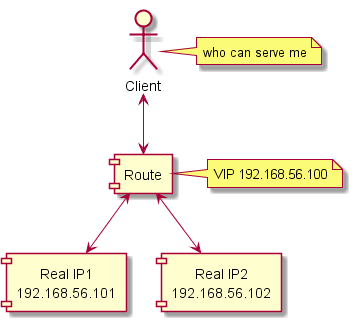
\includegraphics[width=0.5\textwidth]{img/web_topo.png}
  \caption{corosync实验拓扑}
\end{figure}

为了配置一台主机成为HA的节点,通常需要做出如下的准备工作:
\begin{enumerate}[itemsep=0pt,parsep=0pt]
  \item 所有节点的主机名和对应的IP地址解析服务可以正常工作,且每个节点
    的主机名称需要跟“uname -n”命令的结果保持一致;因此,需要保证两个节
    点上的/etc/hosts文件一致;
  \item 两个节点可以基于密钥进行ssh通信;
\end{enumerate}

具体实现为:

\begin{verbatim}
[root@master ~]# cat /etc/hosts
192.168.56.101   master.liucc.com master
192.168.56.102	 slave.liucc.com slave
\end{verbatim}

为了使得重新启动系统后仍能保持如上的主机名称,还需要分别在各节点修改
/etc/sysconfig/network文件。

\begin{verbatim}
master:
# sed -i 's@\(HOSTNAME=\).*@\1master.liucc.com@g'  /etc/sysconfig/network
# hostname master.liucc.com

slave:
# sed -i 's@\(HOSTNAME=\).*@\1slave.liucc.com@g' /etc/sysconfig/network
# hostname slave.liucc.com
\end{verbatim}

各节点生成ssh密钥:

\begin{verbatim}
master:
# cd /root/.ssh
# ssh-keygen -t rsa
# scp id_rsa.pub slave:/root/.ssh/authorized_keys

slave:
# cd /root/.ssh
# ssh-keygen -t rsa
# cat id_rsa.pub >> authorized_keys
# scp authorized_keys master:/root/.ssh
\end{verbatim}

\section{安装软件包}

首先确保已配置本地yum源,然后安装如下依赖包:

\begin{verbatim}
[root@master ~] # yum -y install libibverbs librdmacm lm_sensors \
> libtool-ltdl openhpi-libs openhpi perl-TimeDate
\end{verbatim}

安装完毕依赖包,接下来安装corosync及pacemaker,这里已经准备了相应的软件包,

\begin{verbatim}
[root@master ~]# ls clusterlab
cluster-glue-1.0.6-1.6.el5.i386.rpm       
cluster-glue-libs-1.0.6-1.6.el5.i386.rpm  
corosync-1.2.7-1.1.el5.i386.rpm           
corosynclib-1.2.7-1.1.el5.i386.rpm        
heartbeat-3.0.3-2.3.el5.i386.rpm          
heartbeat-libs-3.0.3-2.3.el5.i386.rpm
libesmtp-1.0.4-5.el5.i386.rpm
pacemaker-1.1.5-1.1.el5.i386.rpm
pacemaker-libs-1.1.5-1.1.el5.i386.rpm
resource-agents-1.0.4-1.1.el5.i386.rpm

[root@master ~]# cd clusterlab
[root@master clusterlab]# yum -y --nogpgcheck localinstall *.rpm
Total size: 17 M
Downloading Packages:
Running rpm_check_debug
Running Transaction Test
Finished Transaction Test
Transaction Test Succeeded
Running Transaction
  Installing     : libesmtp
  Installing     : cluster-glue-libs
  Installing     : corosynclib
  Installing     : cluster-glue
  Installing     : resource-agents 
  Installing     : corosync
  Installing     : heartbeat-libs
  Installing     : pacemaker
  Installing     : pacemaker-libs 
  Installing     : heartbeat
Installed products updated.

Complete!
\end{verbatim}

\section{配置及启动corosync}

下面的配置在master上完成,编辑/etc/corosync/corosync.conf

\begin{verbatim}
[root@master ~]# cd /etc/corosync
[root@master corosync]# cp corosync.conf.example corosync.conf
\end{verbatim}

在文件尾部添加如下内容:

\begin{verbatim}
[root@master corosync]# tail corosync.conf
service {
  ver:  0
  name: pacemaker
}

aisexec {
  user: root
  group:  root
}
\end{verbatim}

并设定此配置文件中 bindnetaddr后面的IP地址为你的网卡所在网络的网络地址,
我们这里的两个节点在192.168.56.0网络,因此这里将其设定为192.168.56.0。
整个配置文件如下:

\begin{verbatim}
[root@master corosync]# cat corosync.conf
# Please read the corosync.conf.5 manual page
compatibility: whitetank

totem {
        version: 2 #版本号
        secauth: off #安全认证
        threads: 0 #线程数,根据CPU个数和核心数确定
        interface {
	        ringnumber: 0 #冗余环号,节点有多个网卡是可定义对应网卡在一个环内
	        bindnetaddr: 192.168.56.0 # 绑定网络地址
	        mcastaddr: 226.94.1.1     # 心跳信息所使用的组播地址
	        mcastport: 5405           # 心跳组播使用的端口
        }
}

logging {
        fileline: off #指定要打印的行
        to_stderr: no #是否发送到标准错误输出
        to_logfile: yes #记录到文件
        to_syslog: yes #记录到syslog
        logfile: /var/log/cluster/corosync.log # corosync日志文件
        debug: off
        timestamp: on #是否打印时间戳,利于定位错误(会消耗CPU资源)
        logger_subsys {
	        subsys: AMF
	        debug: off
        }
}

amf {
        mode: disabled
}

service {
        ver: 0
        name: pacemaker # 定义corosync在启动时自动启动pacemaker
}

aisexec {               # 表示启动corosync的ais功能,以哪个用户身份运行
        user: root
        group: root
}
\end{verbatim}

生成节点间通信时用到的认证密钥文件:

\begin{verbatim}
[root@master corosync]# corosync-keygen
[root@master corosync]# scp -p corosync.conf authkey slave:/etc/corosync

建立corosync日志所需要的目录
[root@master corosync]# mkdir /var/log/cluster
[root@master corosync]# ssh slave "mkdir /var/log/cluster"
\end{verbatim}

接下来就可以启动corosync了,

\begin{verbatim}
[root@master ~]# /etc/init.d/corosync start
Starting Corosync Cluster Engine (corosync):               [  OK  ]
\end{verbatim}

此时,可以查看一下关于corosync引擎是否正常启动的系统日志,

\begin{verbatim}
[root@master corosync]# grep -e "Corosync Cluster Engine" -e "configuration file" /var/log/messages
Feb 28 11:17:02 unionpay smartd[2787]: Opened configuration file /etc/smartd.conf 
Feb 28 11:21:24 master smartd[2770]: Opened configuration file /etc/smartd.conf 
Feb 28 11:44:06 master smartd[2766]: Opened configuration file /etc/smartd.conf 
Feb 28 13:43:05 master corosync[7859]:   [MAIN  ] Corosync Cluster Engine ('1.2.7'): started and ready to provide service.
Feb 28 13:43:05 master corosync[7859]:   [MAIN  ] Successfully read main configuration file '/etc/corosync/corosync.conf'.
\end{verbatim}

查看初始化成员节点通知是否正常发出,
\begin{verbatim}
[root@master corosync]# grep TOTEM /var/log/messages
Feb 28 13:43:05 master corosync[7859]:   [TOTEM ] Initializing transport (UDP/IP).
Feb 28 13:43:05 master corosync[7859]:   [TOTEM ] Initializing transmit/receive security: libtomcrypt SOBER128/SHA1HMAC (mode 0).
Feb 28 13:43:05 master corosync[7859]:   [TOTEM ] The network interface [192.168.56.101] is now up.
Feb 28 13:43:05 master corosync[7859]:   [TOTEM ] A processor joined or left the membership and a new membership was formed.
\end{verbatim}

检查启动过程中是否有错误产生:
\begin{verbatim}
# grep ERROR: /var/log/messages | grep -v unpack_resources
\end{verbatim}

查看pacemaker是否正常启动:
\begin{verbatim}
[root@master corosync]#  grep pcmk_startup /var/log/messages
Feb 28 13:43:05 master corosync[7859]:   [pcmk  ] info: pcmk_startup: CRM: Initialized
Feb 28 13:43:05 master corosync[7859]:   [pcmk  ] Logging: Initialized pcmk_startup
Feb 28 13:43:05 master corosync[7859]:   [pcmk  ] info: pcmk_startup: Maximum core file size is: 4294967295
Feb 28 13:43:05 master corosync[7859]:   [pcmk  ] info: pcmk_startup: Service: 9
Feb 28 13:43:05 master corosync[7859]:   [pcmk  ] info: pcmk_startup: Local hostname: master.liucc.com
\end{verbatim}

如果上面命令执行均没有问题,接着可以执行如下命令启动node2上的corosync
\begin{verbatim}
[root@slave cluster]# ssh slave -- /etc/init.d/corosync start
The authenticity of host 'slave (192.168.56.102)' can't be established.
RSA key fingerprint is 3e:36:02:7a:4c:3c:0d:39:d0:51:a4:86:0f:85:97:c8.
Are you sure you want to continue connecting (yes/no)? yes
Warning: Permanently added 'slave' (RSA) to the list of known hosts.
Starting Corosync Cluster Engine (corosync): [  OK  ]
[root@slave cluster]# ssh slave -- /etc/init.d/corosync status
corosync (pid  10867) is running...
\end{verbatim}

注意:启动node2需要在node1上使用如上命令进行,不要在node2节点上直接启动;

使用如下命令查看集群节点的启动状态:
\begin{verbatim}
[root@master corosync]# crm status
============
Last updated: Sat Feb 28 13:48:11 2015
Stack: openais
Current DC: master.liucc.com - partition with quorum
Version: 1.1.5-1.1.el5-01e86afaaa6d4a8c4836f68df80ababd6ca3902f
2 Nodes configured, 2 expected votes
0 Resources configured.
============

Online: [ master.liucc.com slave.liucc.com ]

\end{verbatim}

从上面的信息可以看出两个节点都已经正常启动,并且集群已经处于正常工作状
态。

由于corosync默认启用了stonith,而当前集群并没有相应的stonith设备,因此
此默认配置目前尚不可用,这可以通过如下命令验正:

\begin{verbatim}
[root@master corosync]# crm_verify -L
crm_verify[7926]: 2015/02/28_13:51:01 ERROR: unpack_resources: Resource start-up disabled since no STONITH resources have been defined
crm_verify[7926]: 2015/02/28_13:51:01 ERROR: unpack_resources: Either configure some or disable STONITH with the stonith-enabled option
crm_verify[7926]: 2015/02/28_13:51:01 ERROR: unpack_resources: NOTE: Clusters with shared data need STONITH to ensure data integrity
Errors found during check: config not valid
  -V may provide more details

\end{verbatim}

我们里可以通过如下命令先禁用stonith:

\begin{verbatim}
[root@master corosync]# crm configure property stonith-enabled=false
\end{verbatim}

使用如下命令查看当前的配置信息:

\begin{verbatim}
[root@master corosync]# crm configure show
node master.liucc.com
node slave.liucc.com
property $id="cib-bootstrap-options" \
	dc-version="1.1.5-1.1.el5-01e86afaaa6d4a8c4836f68df80ababd6ca3902f" \
	cluster-infrastructure="openais" \
	expected-quorum-votes="2" \
	stonith-enabled="false"
\end{verbatim}

从中可以看出stonith已经被禁用。上面的crm,crm\_verify命令是1.0后的版本的
pacemaker提供的基于命令行的集群管理工具;可以在集群中的任何一个节点上执
行。

\section{为集群添加资源}

corosync支持heartbeat,LSB和ocf等类型的资源代理,目前较为常用的类型为
LSB和OCF两类,stonith类专为配置stonith设备而用;可以通过如下命令查看当
前集群系统所支持的类型:

\begin{verbatim}
# crm ra classes 
heartbeat
lsb
ocf / heartbeat pacemaker
stonith
\end{verbatim}

如果想要查看某种类别下的所用资源代理的列表,可以使用类似如下命令实现:

\begin{verbatim}
[root@master ~]# crm ra list lsb
NetworkManager      acpid               anacron             apmd                atd                 auditd              autofs
avahi-daemon        avahi-dnsconfd      bluetooth           capi                conman              corosync            cpuspeed
crond               cups                cups-config-daemon  dnsmasq             dund                firstboot           functions
gpm                 haldaemon           halt                heartbeat           hidd                hplip               httpd
ip6tables           ipmi                iptables            irda                irqbalance          iscsi               iscsid
isdn                kdump               killall             krb524              kudzu               lm_sensors          logd
lvm2-monitor        mcstrans            mdmonitor           mdmpd               messagebus          microcode_ctl       multipathd
mysqld              netconsole          netfs               netplugd            network             nfs                 nfslock
nscd                ntpd                openhpid            openibd             pacemaker           pand                pcscd
portmap             postgresql-9.0      psacct              rawdevices          rdisc               readahead_early     readahead_later
restorecond         rhnsd               rhsmcertd           rpcgssd             rpcidmapd           rpcsvcgssd          saslauthd
sendmail            setroubleshoot      single              smartd              snmpd               snmptrapd           sshd
syslog              sysstat             tomcat              vboxadd             vboxadd-service     vboxadd-x11         vncserver
vsftpd              wdaemon             winbind             wpa_supplicant      xfs                 xinetd              ypbind
yum-updatesd

[root@master ~]# crm ra list ocf heartbeat
AoEtarget           AudibleAlarm        CTDB                ClusterMon          Delay               Dummy               EvmsSCC
Evmsd               Filesystem          ICP                 IPaddr              IPaddr2             IPsrcaddr           IPv6addr
LVM                 LinuxSCSI           MailTo              ManageRAID          ManageVE            Pure-FTPd           Raid1
Route               SAPDatabase         SAPInstance         SendArp             ServeRAID           SphinxSearchDaemon  Squid
Stateful            SysInfo             VIPArip             VirtualDomain       WAS                 WAS6                WinPopup
Xen                 Xinetd              anything            apache              conntrackd          db2                 drbd
eDir88              exportfs            fio                 iSCSILogicalUnit    iSCSITarget         ids                 iscsi
jboss               ldirectord          mysql               mysql-proxy         nfsserver           nginx               oracle
oralsnr             pgsql               pingd               portblock           postfix             proftpd             rsyncd
scsi2reservation    sfex                syslog-ng           tomcat              vmware 

[root@master ~]# crm ra list ocf pacemaker
ClusterMon    Dummy         HealthCPU     HealthSMART   Stateful      SysInfo       SystemHealth  controld      o2cb          ping
pingd      

[root@master ~]# crm ra list stonith
apcmaster               apcmastersnmp           apcsmart                baytech                 bladehpi                cyclades
external/drac5          external/dracmc-telnet  external/hmchttp        external/ibmrsa         external/ibmrsa-telnet  external/ipmi
external/ippower9258    external/kdumpcheck     external/rackpdu        external/riloe          external/sbd            external/vmware
external/xen0           external/xen0-ha        fence_legacy            ibmhmc                  ipmilan                 meatware
nw_rpc100s              rcd_serial              rps10                   suicide                 wti_mpc                 wti_nps
\end{verbatim}

\begin{verbatim}
# crm ra info [class:[provider:]]resource_agent
例如:
[root@master ~]# crm ra info ocf:heartbeat:IPaddr
Manages virtual IPv4 addresses (portable version) (ocf:heartbeat:IPaddr)

This script manages IP alias IP addresses
It can add an IP alias, or remove one.

Parameters (* denotes required, [] the default):

ip* (string): IPv4 address
    The IPv4 address to be configured in dotted quad notation, for example
    "192.168.1.1".

nic (string, [eth0]): Network interface
    The base network interface on which the IP address will be brought
    online.
    
    If left empty, the script will try and determine this from the
    routing table.
    
    Do NOT specify an alias interface in the form eth0:1 or anything here;
    rather, specify the base interface only.
    
    Prerequisite:
    
    There must be at least one static IP address, which is not managed by
    the cluster, assigned to the network interface.
    
    If you can not assign any static IP address on the interface,
    modify this kernel parameter:
    sysctl -w net.ipv4.conf.all.promote_secondaries=1
    (or per device)

cidr_netmask (string): Netmask
    The netmask for the interface in CIDR format. (ie, 24), or in
    dotted quad notation  255.255.255.0).
    
    If unspecified, the script will also try to determine this from the
    routing table.

broadcast (string): Broadcast address
    Broadcast address associated with the IP. If left empty, the script will
    determine this from the netmask.

iflabel (string): Interface label
    You can specify an additional label for your IP address here.

lvs_support (boolean, [false]): Enable support for LVS DR
    Enable support for LVS Direct Routing configurations. In case a IP
    address is stopped, only move it to the loopback device to allow the
    local node to continue to service requests, but no longer advertise it
    on the network.

local_stop_script (string): 
    Script called when the IP is released

local_start_script (string): 
    Script called when the IP is added

ARP_INTERVAL_MS (integer, [500]): milliseconds between gratuitous ARPs
    milliseconds between ARPs

ARP_REPEAT (integer, [10]): repeat count
    How many gratuitous ARPs to send out when bringing up a new address

ARP_BACKGROUND (boolean, [yes]): run in background
    run in background (no longer any reason to do this)

ARP_NETMASK (string, [ffffffffffff]): netmask for ARP
    netmask for ARP - in nonstandard hexadecimal format.

Operations' defaults (advisory minimum):

    start         timeout=20s
    stop          timeout=20s
    monitor       interval=5s timeout=20s
\end{verbatim}

\section{为Web创建IP资源}

接下来要创建的web集群创建一个IP地址资源,以在通过集群提供web服务时使用;
这可以通过如下方式实现:

语法:

\begin{verbatim}
primitive <rsc> [<class>:[<provider>:]]<type>
          [params attr_list]
          [operations id_spec]
            [op op_type [<attribute>=<value>...] ...]

op_type :: start | stop | monitor
\end{verbatim}

例子:

\begin{verbatim}
 primitive apcfence stonith:apcsmart \
          params ttydev=/dev/ttyS0 hostlist="node1 node2" \
          op start timeout=60s \
          op monitor interval=30m timeout=60s
\end{verbatim}


\section{高可用验证}

\chapter{DRBD}
\label{chap:drbd}

distributed replicated block device

a software-based, shared-nothing, replicated storage solution
mirroring the content of block devices (hard disks, partitions,
logical volumes etc.) between servers.

DRBD's core functionality is implemented by way of a Linux Kernel
module.

User space administration tools

drbdadm

The high-level administration tool of the DRBD program suite. It
obtains all DRBD configuration parameters from the configuration 
file /etc/drbd.conf

drbdsetup

The program that allows users to configure the DRBD module that has
been loaded into the running kernel. It is the low-level tool within
the DRBD program suite.

Resource roles

In DRBD, every resource has a role, which may be Primary or Secondary.

Primary

A DRBD device in the primary role can be used unrestrictedly for read
and write operations. It may be used for creating and mounting file
systems, raw or direct I/O to the block device, etc.

Secondary

A DRBD device in the secondary role receives all updates from the perr
node's device, but otherwise disallows access completely.  It can not
be used by applications, neither for read nor write access.

DRBD modes

Single-primary mode
\begin{quote}
Any resource is, at any given time, in the primary role on only one
cluster member.

Only one cluster node manipulates the data at any moment.

This mode can be used with any conventional file system (ext3, ext4,
XFS, etc.)

Deploying DRBD in single-primary mode is the canonical approach for
high availability (fail-over capable) clusters.
\end{quote}

Dual-primary mode
\begin{quote}
Any resource is, at any given time, in the primary role on both
cluster nodes.

Since concurrent access to the data is thus possible, this mode
requires the use of a shared cluster file system that utilizes a
distributed lock manager. Examples include GFS and OCFS2.

Deploying DRBD in dual-primary mode is the preferred approach for
load-balancing clusters which require concurrent data access from two
nodes.

Disabled by default, and must be enabled explicitly in DRBD's
configuration file.

Available in DRBD 8.0 and later.
\end{quote}
 
\section{三种同步模式}

\begin{enumerate}[itemsep=0pt,parsep=0pt]
\item 协议A
\begin{quote}
异步复制协议。只要主节点完成本地写操作就认为写操作完成,并且需要复制的
数据包会被存储到本地TCP发送缓冲中。当发生failover故障,数据可能会丢失。
当发生failover故障时,在备节点的数据被认为仍是稳固的,然而,在crash发生
的时间点上很多最新的更新操作会丢失。
\end{quote}

\item 协议B
\begin{quote}
内存同步(半同步)复制协议。当本地盘的写已经完成,并且复制数据包已经到
达对应从节点,此时主节点才认为磁盘写已经完成。通常情况下,发生failover
不会导致数据丢失(因为后备系统内存中已经获得了数据更新)。然而,如果所
有节点同时出现电源故障,则主节点数据存储会产生不可逆的错误结构,主节点
上多数最新写入的数据可能会丢失。
\end{quote}

\item 协议C
\begin{quote}
同步复制协议。只有在本地和远程磁盘都确定写入已经完成时,主节点才会认为
写入完成。这样可确保发生故障时不会导致任何数据丢失。如果发生数据丢失的
现象,那也只会在所有节点同时存在错误存储时才会发生。
\end{quote}
\end{enumerate}

Efficient synchronization
\begin{quote}
Synchronization is necessary if the replication link has been
interrupted for any reason

1. failure of the primary node
2. failure of the secondary node
3. or interruption of the replication link

(Re-)synchronization is distinct from device replication
\end{quote}

Split brain
\begin{quote}
Split brain is a situation where, due to temporary failure of all
network links between cluster nodes, and possibly due to intervension
by a cluster management software or human error, both nodes switched
to the primary role while disconnected.
\end{quote}

automatic recovery
\begin{quote}
DRBD allows for automatic operator notification (by email or other
means) when it detects split brain.

DRBD has several resolution algorithms available for resolving the
split brain automaticly.

1. Discarding modifications made on the "younger" primary
2. Discarding modifications made on the "older" primary
3. Discarding modifications on the primary with fewer changes
4. Graceful recovery from split brain if one host has had no intermediate changes
\end{quote}

\section{安装及配置DRBD}

DRBD包含两大主要组件,内核空间中的驱动代码与用户空间中的管理工具。自从
Linux内核2.6.33版本及之后版本,DRBD的驱动代码已整合进了内核模块。所以,
在2.6.33版本及更新版本后,我们只需要安装用户空间的管理工具即可。否则,
我们需要同时安装内核支持模块与管理工具两个包,并且两个工具的版本号要保
持一致。

实验环境:

\begin{figure}[!h]
\centering
\begin{tabular}{llll}
\toprule
机器列表        & IP地址        & 操作系统       & DRBD版本 \\
\midrule
node1.laven.com & 192.168.1.15  & RHEL5U5 32bit  & 8.3.8 \\
node2.laven.com & 192.168.1.16  & RHEL5U5 32bit  & 8.3.8 \\
\bottomrule
\end{tabular}
\end{figure}


开始安装

\small{
\begin{verbatim}
[root@node1 ~]# ls
drbd83-8.3.8-1.el5.centos.i386.rpm
kmod-drbd83-8.3.8-1.el5.centos.i386.rpm

[root@node1 ~]# rpm -ivh kmod-drbd83-8.3.8-1.el5.centos.i386.rpm
[root@node1 ~]# rpm -ivh drbd83-8.3.8-1.el5.centos.i386.rpm
\end{verbatim}
}
\normalsize

在node2上进行同样的安装操作。

开始配置,

\small{
\begin{verbatim}
[root@node1 ~]# ls
drbd83-8.3.8-1.el5.centos.i386.rpm
kmod-drbd83-8.3.8-1.el5.centos.i386.rpm

[root@node1 ~]# rpm -ivh kmod-drbd83-8.3.8-1.el5.centos.i386.rpm
[root@node1 ~]# rpm -ivh drbd83-8.3.8-1.el5.centos.i386.rpm
\end{verbatim}
}
\normalsize

安装完成之后,来个简单的配置,使drbd可以简单的用起来。drbd的主配置文件
为/etc/drbd.conf,其中还有一个/etc/drbd.d目录,里面放置了其他的配置文件,
这也是便于管理,因此,我们可以分段进行配置,然后放置到该目录即可,在主
配置文件中使用include指令把这些文件加载进来即可。

看一下全局配置文件,

\small{
\begin{verbatim}
[root@node1 ~]# cat /etc/drbd.d/global_common.conf 
global {
   usage-count no;
   # minor-count dialog-refresh disable-ip-verification
}

common {
   protocol C;

   handlers {
      pri-on-incon-degr "/usr/lib/drbd/notify-pri-on-incon-degr.sh; \
      /usr/lib/drbd/notify-emergency-reboot.sh; \
      echo b > /proc/sysrq-trigger ; reboot -f";

      pri-lost-after-sb "/usr/lib/drbd/notify-pri-lost-after-sb.sh; \
      /usr/lib/drbd/notify-emergency-reboot.sh; \
      echo b > /proc/sysrq-trigger ; reboot -f";

      local-io-error "/usr/lib/drbd/notify-io-error.sh; \
      /usr/lib/drbd/notify-emergency-shutdown.sh; \
      echo o > /proc/sysrq-trigger ; halt -f";

      fence-peer "/usr/lib/drbd/crm-fence-peer.sh";
      split-brain "/usr/lib/drbd/notify-split-brain.sh root";
      out-of-sync "/usr/lib/drbd/notify-out-of-sync.sh root";
      before-resync-target "/usr/lib/drbd/snapshot-resync-target-lvm.sh \
      -p 15 -- -c 16k";
       after-resync-target /usr/lib/drbd/unsnapshot-resync-target-lvm.sh;
   }

   startup {
       wfc-timeout 120;
       degr-wfc-timeout 120;
   }

   disk {
       on-io-error detach;
       fencing resource-only;
   }

   net {
       cram-hmac-alg "sha1";
       shared-secret "mypass";
   }

   syncer {
       rate 100M;
   }
}
\end{verbatim}
}
\normalsize

现在定一个简单的资源r0,资源文件后缀以res结尾。

\small{
\begin{verbatim}
[root@node1 ~]# cat /etc/drbd.d/r0.res 
resource r0 {
  on node1.laven.com {
    device    /dev/drbd0;
    disk      /dev/sdb1;
    address   192.168.1.15:7789;
    meta-disk internal;
  }

  on node2.laven.com {
    device    /dev/drbd0;
    disk      /dev/sdb1;
    address   192.168.1.16:7789;
    meta-disk internal;
  }
}
\end{verbatim}
}
\normalsize

配置完毕,我们可以把这些文件复制到节点node2上去,

\small{
\begin{verbatim}
[root@node1 ~]# scp /etc/drbd.d/* node2:/etc/drbd.d/
\end{verbatim}
}
\normalsize

好了,初始化两端的drbd,然后启动drbd服务。

\small{
\begin{verbatim}
[root@node1 ~]# drbdadm create-md r0
[root@node2 ~]# drbdadm create-md r0
\end{verbatim}
}
\normalsize

初始化完毕之后,我们把node1作为主节点,node2作为从节点。之后,我们把
/dev/drbd0格式化然后挂载到/web目录下,然后在/web路下创建一些文件,然后
到node2上检查这些文件是否可以看到。

\small{
\begin{verbatim}
[root@node1 ~]# fdisk /dev/sdb -> /dev/sdb1
[root@node1 ~]# mke2fs -j /dev/drbd0
[root@node1 ~]# mount /dev/drbd0 /web
[root@node1 ~]# drbdadm primary r0
[root@node1 ~]# cd /web
[root@node1 web]# for i in {1..10}; do echo "Hello, world" > file${i}; \
> done
[root@node1 web]# ls
file1  file10  file2  file3  file4  file5  
file6  file7   file8  file9  lost+found
\end{verbatim}
}
\normalsize

这时,我们把node2作为主节点,并把/dev/drbd0挂载到/web目录下,验证是不是
有上述文件。首先,需要把/web目录umount,然后把node1变为从节点。之后,
node2需要先把自己变为主节点,然后挂载/dev/drbd0到/web下即可,

\small{
\begin{verbatim}
[root@node1 ~]# umount /web
[root@node1 ~]# drbdadm secondary r0
[root@node2 ~]# drbdadm primary r0
[root@node2 ~]# mount /dev/drbd0 /web
[root@node2 ~]# ls /web
file1  file10  file2  file3  file4  file5  
file6  file7   file8  file9  lost+found
[root@node2 ~]# cat /web/file*
Hello, world
Hello, world
Hello, world
Hello, world
Hello, world
Hello, world
Hello, world
Hello, world
Hello, world
Hello, world
\end{verbatim}
}
\normalsize

\chapter{HAproxy负载均衡与高可用}
\label{chap:haproxyCluster}

\section{关于HAproxy}
\label{sec:aboutHaproxy}

HAproxy提供高可用性、负载均衡以及基于TCP和HTTP应用的代理,支持虚拟主机,
它是免费、快速并且可靠的一种解决方案。HAproxy特别适用于那些负载特大
的web站点,这些站点通常又需要会话保持或七层处理。HAProxy运行在当前的硬
件上,完全可以支持数以万计的并发连接。并且它的运行模式使得它可以很简单
安全的整合进您当前的架构中, 同时可以保护你的web服务器不被暴露到网络
上。

HAproxy实现了一种事件驱动, 单一进程模型,此模型支持非常大的并发连接数。
多进程或多线程模型受内存限制 、系统调度器限制以及无处不在的锁限制,很少
能处理数千并发连接。事件驱动模型因为在有更好的资源和时间管理的用户空
间(User-Space) 实现所有这些任务,所以没有这些问题。此模型的弊端是,在多
核系统上,这些程序通常扩展性较差。这就是为什么他们必须进行优化以 使每
个CPU时间片(Cycle)做更多的工作。\cite{baike}

\section{环境准备}
\label{sec:envPrepareHaproxy}

\subsection{测试环境准备}

\subsection{安装EPEL源}

\section{HAproxy的高可用}
\label{sec:HighAvailableHaproxy}


